%
% main.tex -- Paper zum Thema <zeta>
%
% (c) 2020 Autor, OST Ostschweizer Fachhochschule
%
% !TEX root = ../../buch.tex
% !TEX encoding = UTF-8
%
\chapter{Die Summe aller natürlichen Zahlen und die riemannsche Zeta-Funktion\label{chapter:zeta}}
\kopflinks{Die Summe aller natürlichen Zahlen und die riemannsche Zeta-Funktion}
\begin{refsection}
\chapterauthor{Melissa Haumüller}

Ein paar Hinweise für die korrekte Formatierung des Textes
\begin{itemize}
\item
Absätze werden gebildet, indem man eine Leerzeile einfügt.
Die Verwendung von \verb+\\+ ist nur in Tabellen und Arrays gestattet.
\item
Die explizite Platzierung von Bildern ist nicht erlaubt, entsprechende
Optionen werden gelöscht. 
Verwenden Sie Labels und Verweise, um auf Bilder hinzuweisen.
\item
Beginnen Sie jeden Satz auf einer neuen Zeile. 
Damit ermöglichen Sie dem Versionsverwaltungssysteme, Änderungen
in verschiedenen Sätzen von verschiedenen Autoren ohne Konflikt 
anzuwenden.
\item 
Bilden Sie auch für Formeln kurze Zeilen, einerseits der besseren
Übersicht wegen, aber auch um GIT die Arbeit zu erleichtern.
\end{itemize}

%
% einleitung.tex -- Beispiel-File für die Einleitung
%
% (c) 2020 Prof Dr Andreas Müller, Hochschule Rapperswil
%
% !TEX root = ../../buch.tex
% !TEX encoding = UTF-8
%
\section{Einleitung\label{Einleitung}}

Die Frage nach der Summe aller natürlichen Zahlen gehört zu den faszinierendsten und zugleich missverständlichsten Themen der modernen Mathematik. 
Auf den ersten Blick scheint die Reihe 
1 + 2 + 3 + 4 + \dots
offensichtlich gegen Unendlich zu divergieren. 
Dennoch taucht in verschiedenen mathematischen und physikalischen Kontexten die überraschende Aussage auf, diese Summe sei gleich 
\[
-\frac{1}{12}.
\]
Ziel dieses Papers ist es, diesen scheinbaren Widerspruch aufzulösen, indem der Begriff der Konvergenz präzisiert, die Riemannsche Zeta-Funktion eingeführt und deren analytische Fortsetzung untersucht wird. 
Abschliessend wird bewertet, in welchem Sinne die Zuordnung des Wertes
\[
-\frac{1}{12}
\] 
sinnvoll ist. 

%
% teil1.tex -- Beispiel-File für das Paper
%
% (c) 2020 Prof Dr Andreas Müller, Hochschule Rapperswil
%
% !TEX root = ../../buch.tex
% !TEX encoding = UTF-8
%
\section{Teil 1
\label{zeta:section:teil1}}

\section{Konvergente und divergente Reihen
\label{konvergente-und-divergente-reihen}}

Um die analytische Fortsetzung zu verstehen, muss man sich zuerst mit den Begriffen der konvergenten und divergenten Reihen auskennen.

Unendliche Summen sind Reihen. 
Hierbei gibt es drei Verhaltensweisen, wie sich eine Reihe verhalten kann.

Ist eine reihe konvergent wie zum Beispiel

\[
1 + \frac{1}{2} + \frac{1}{4} + \frac{1}{8} + \frac{1}{16} + \ldots = 2,
\]

so bekommen wir ein endliches Resultat, da die Funktion der Teilsummen irgendwann gegen Null geht.

Ist eine Reihe bestimmt divergent wie zum Beispiel

\[
\sum_{n=1}^{\infty} 1 = 1 + 1 + 1 + 1 + \ldots
\]

oder

\[
1 - \sum_{n=1}^{\infty} 1 = 1 - 1 - 1 - 1 - \ldots,
\]

so geht die Summe entweder gegen Unendlich oder gegen minus Unendlich.

Ist eine Reihe unbestimmt divergent wie zum Beispiel

\[
\sum_{n=0}^{\infty} (-1)^n = 1 - 1 + 1 - 1 + \ldots,
\]

so alterniert das Ergebnis immer und ist somit undefiniert.

Die Summe aller natürlichen Zahlen ist offensichtlich bestimmt divergent. 
Es werden immer grösser werdende Zahlen addiert und somit geht das Ergebnis gegen Unendlich.


%
% teil2.tex -- Beispiel-File für teil2 
%
% (c) 2020 Prof Dr Andreas Müller, Hochschule Rapperswil
%
% !TEX root = ../../buch.tex
% !TEX encoding = UTF-8
%
\section{Riemannsche Zeta-Funktion}\label{Riemannsche Zeta-Funktion}

Die Riemannsche Zeta-Funktion wurde 1859 von Bernhard Riemann untersucht und ist eine zentrale Funktion der
analytischen Zahlentheorie. Sie wird üblicherweise als unendliche Reihe
definiert. Für alle komplexen Variablen s mit Realteil grösser als 1
ergibt sich ihre Darstellung als
\[
\zeta(s) = \sum_{n = 1}^{\infty}\frac{1}{n^{s}}.
\]
Diese Definition beschreibt eine Dirichlet-Reihe, deren Konvergenz für Re(s) \textgreater{} 1 gewährleistet ist. 
Bereits in diesem Definitionsbereich zeigt die Funktion bemerkenswerte Eigenschaften. 
So nimmt sie für bestimmte Argumente konkrete Werte an:

\begin{table}[h]
	\centering
	\begin{tabular}{|c|c|c|}
		\hline
		\rowcolor{blue!40}
		\textcolor{white}{\textbf{\textit{s}}} & 
		\textcolor{white}{\textbf{$\zeta(s)$}} & 
		\textcolor{white}{\textbf{Ungefährer Wert}} \\
		\hline
		$2$ & $\pi^2/6$ & $\approx 1{,}6449$ \\
		\hline
		$4$ & $\pi^4/90$ & $\approx 1{,}0823$ \\
		\hline
		$-1$ & $-1/12$ & (analytische Fortsetzung) \\
		\hline
		$0$ & $-1/2$ & (analytische Fortsetzung) \\
		\hline
	\end{tabular}
	\caption{Ausgewählte Werte der Zeta-Funktion}
	\label{tab:zeta}
\end{table}

Besonders bemerkenswert ist hier der Wert $\zeta$(2) = $\frac{\pi^2}{6}$, den Euler bereits 1735 nachwies, bekannt als das Basler Problem. 
Die letzen beiden Zeilen der Tabelle gehören jedoch nicht zum ursprünglichen Definitionsbereich (s > 1), sondern sind nur durch analytische Fortsetzung erreichbar. 

\begin{figure}
	\centering
	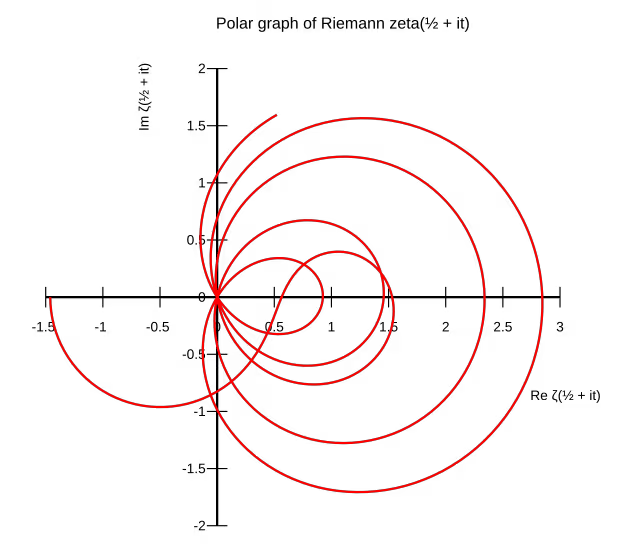
\includegraphics[width=0.7\linewidth]{papers/zeta/Abbildung_Zeta.png}
	\caption{}
	\label{fig:abbildungzeta}
\end{figure}

Die spiralförmige Darstellung in Abbildung \ref{fig:abbildungzeta} zeigt den Verlauf der Zeta-Funktion $\zeta$(s) in der komplexen Ebene, wobei s entlang einer vertikalen Linie mit festem Realteil variiert. Die Schnittpunkte der Kurve mit dem Ursprung (sichtbar als die Stellen, an denen die Spirale durch den Mittelpunkt verläuft) entsprechen den sogenannten nicht-trivialen Nullstellen der Zeta-Funktion. Diese liegen alle auf der Linie Re(s) = $\frac{1}{2}$ und sind Gegenstand der berühmten, bis heute unbewiesenen Riemannschen Vermutung, einem der bedeutendsten offenen Probleme der Mathematik. 

Nützlich ist die Riemannsche Zeta-Funktion ebenfalls, um eine Annäherung der Primzahlfunktion zu schaffen. 
Das Euler-Produkt
\[
\zeta(s) = \prod_{p \ \text{prim}} \frac{1}{1 - p^{-s}}
\]
beschreibt eine geometrische Reihe,welche den Zusammenhang aller Primzahlen aufzeigt. 

\begin{figure}
	\centering
	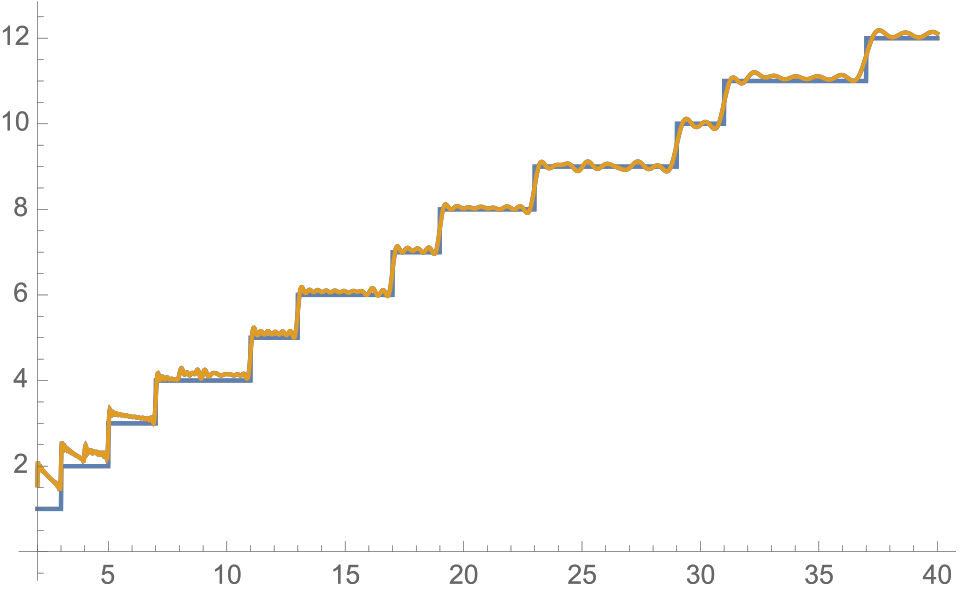
\includegraphics[width=0.7\linewidth]{papers/zeta/Primzahlen.png}
	\caption{}
	\label{fig:primzahlen}
\end{figure}

Die blaue Treppenkurve in Abbildung \ref{fig:primzahlen} zeigt die Primzahlzählfunktion $\pi$(x), welche für jede reelle Zahl x angibt, wie viele Primzahlen kleiner oder gleich x existieren. Die orangefarbene Kurve stellt den Logarithmischen Integralausdruch Li(x) dar. Das ist eine von Riemann entwickelte Näherungsformel für $\pi$(x), die direkt aus der Zeta-Funktion abgeleitet wird. Man erkennt deutlich, wie eng beide Kurven beieinander liegen: Li(x) approximiert die Verteilung der Primzahlen mit bemerkenswertet Genauigkeit, selbst für kleine Werte von x.



% Für was wird die Zeta-funktion angewendet in der Praxis? -> Verteilung von Primzahlen, analytische Zahlentheorie, mathematische Physik und Wahrscheinlichkeit und Statistik
% Text zum Bild schreiben
% Abstimmen auf Text vom Theorieteil des Buches von Herr Müller. Erweiterung mit Primzahl-Funktion. 


%
% teil3.tex -- Beispiel-File für Teil 3
%
% (c) 2020 Prof Dr Andreas Müller, Hochschule Rapperswil
%
% !TEX root = ../../buch.tex
% !TEX encoding = UTF-8
%
\section{Analytische Fortsetzung
\label{Analytische Fortsetzung}}

Die analytische Fortsetzung ist ein Konzept aus der komplexen Analysis.
Im Grunde genommen kann durch sie eine Funktion erweitert werden
ausserhalb ihres Definitionsbereiches.

Voraussetzung dafür ist lediglich, dass die Funktion holomorph ist.

Grundsätzlich wird in der Analytischen Fortsetzung einfach eine neue Funktion konstruiert, die den selben Definitionsbereich wie die ursprüngliche Funktion hat. 
Jedoch ist diese neue Funktion auch ausserhalb dieses Bereichs definiert.

In der Anwendung auf die Riemannsche Zeta-Funktion kann eine solche analytische Fortsetzung fast auf die gesamte komplexe Ebene angewendet werden. 
Die einzige Ausnahme ist der Punkt bei s = 1.

%
%

\subsection{Anwendung auf die Zeta-Funktion\label{Anwendung auf die Zeta-Funktion}}

Beispielsweise wenn man die Zeta-Funktion anschaut mit

\[\zeta(s) = 1 + \frac{1}{2^{s}} + \frac{1}{3^{s}} + \frac{1}{4^{s}} + \ldots\]

, so ist diese nur korrekt für alle Zahlen \textgreater{} 1.

Wenn man jedoch dann die Analytische Fortsetzung verwendet und die Funktion anders darstellt durch eine Erweiterung des Terms, bekommt man

\[\zeta(s) = \frac{1}{{1 - 2}^{1 - s}}(1 + \frac{1}{2^{s}} + \frac{1}{3^{s}} + \frac{1}{4^{s}} + \ldots),\]

was nun schon korrekt ist für alle Zahlen \textgreater{} 0.

Die Formel wird nun erweitert, bis man

\[\zeta(s) = 2^s \pi^{s-1} \sin\left(\frac{\pi s}{2}\right) \Gamma(1 - s)\,\zeta(1 - s)\].

hat. 
So ist sie definiert für auch fast alle negativen Werte für s. 
Wenn man für s jetzt -1 einsetzt, so kommt man mit den Umformungen von

\[\zeta(-1) = 2^{-1} \pi^{-2} \sin\left(-\frac{\pi}{2}\right)\Gamma(2)\zeta(2)\].

auf

\[\sin\left(-\frac{\pi}{2}\right) = -1, \quad \Gamma(2) = 1! = 1, \quad \zeta(2) = \frac{\pi^2}{6}\].

und schlussendlich auf

\[
\frac{1}{2} \cdot \frac{1}{\pi^2} \cdot (-1) \cdot 1 \cdot \frac{\pi^2}{6} = -\frac{1}{12},
\]
was
\[
-\frac{1}{12}
\] ergibt. 

%Berechnung und analytische Fortsetzung noch besser beschreiben, auch Zusammenhang mit komplexen Zahlen näher erklären.



%
% teil3.tex -- Beispiel-File für Teil 3
%
% (c) 2020 Prof Dr Andreas Müller, Hochschule Rapperswil
%
% !TEX root = ../../buch.tex
% !TEX encoding = UTF-8
%
\section{Fazit
\label{Fazit}}

Die Aussage, dass die Summe aller natürlichen Zahlen -1/12 ist, macht
auf den Ersten Blick keinen Sinn, da die Reihe offensichtlich
divergiert. Dennoch ist der Wert -1/12 im Rahmen der analytischen
Fortsetzung der Zeta-Funktion mathematisch belegt und sinnvoll
definiert.

Bei dem Ergebnis, das man von der analytischen Fortsetzung der
Riemannschen Zeta-Funktion erhält, handelt es sich jedoch nicht um eine
Summe im herkömmlichen Sinn. Es ist eher als erweiterte Interpretation
zu betrachten, die in mathematischen Kontexten nützlich ist.




\printbibliography[heading=subbibliography]
\end{refsection}
